\documentclass[a4paper]{book}
\usepackage{makeidx}
\usepackage{natbib}
\usepackage{graphicx}
\usepackage{multicol}
\usepackage{float}
\usepackage{listings}
\usepackage{color}
\usepackage{ifthen}
\usepackage[table]{xcolor}
\usepackage{textcomp}
\usepackage{alltt}
\usepackage{ifpdf}
\ifpdf
\usepackage[pdftex,
            pagebackref=true,
            colorlinks=true,
            linkcolor=blue,
            unicode
           ]{hyperref}
\else
\usepackage[ps2pdf,
            pagebackref=true,
            colorlinks=true,
            linkcolor=blue,
            unicode
           ]{hyperref}
\usepackage{pspicture}
\fi
\usepackage[utf8]{inputenc}
\usepackage{mathptmx}
\usepackage[scaled=.90]{helvet}
\usepackage{courier}
\usepackage{sectsty}
\usepackage[titles]{tocloft}
\usepackage{doxygen}
\lstset{language=C++,inputencoding=utf8,basicstyle=\footnotesize,breaklines=true,breakatwhitespace=true,tabsize=8,numbers=left }
\makeindex
\setcounter{tocdepth}{3}
\renewcommand{\footrulewidth}{0.4pt}
\renewcommand{\familydefault}{\sfdefault}
\hfuzz=15pt
\setlength{\emergencystretch}{15pt}
\hbadness=750
\tolerance=750
\begin{document}
\hypersetup{pageanchor=false,citecolor=blue}
\begin{titlepage}
\vspace*{7cm}
\begin{center}
{\Large \-Login-\/\-Authorization }\\
\vspace*{1cm}
{\large \-Generated by Doxygen 1.7.6.1}\\
\vspace*{0.5cm}
{\small Wed Jul 2 2014 13:20:49}\\
\end{center}
\end{titlepage}
\clearemptydoublepage
\pagenumbering{roman}
\tableofcontents
\clearemptydoublepage
\pagenumbering{arabic}
\hypersetup{pageanchor=true,citecolor=blue}
\chapter{\-Getting \-Started}
\label{index}\hypertarget{index}{}\hypertarget{index_sec_1}{}\section{\-Installation}\label{index_sec_1}
\-To get started right away, read the chapter on \hyperlink{install}{\-Installation} .\hypertarget{index_sec_2}{}\section{\-Oauth 2.\-0}\label{index_sec_2}
\-If you want to learn the basics of \-O\-Auth 2.\-0 consider reading the \hyperlink{oauth}{\-Overview of \-O\-Auth 2.\-0} .\hypertarget{index_sec_3}{}\section{\-A\-P\-I Documentation}\label{index_sec_3}
\-To see a full \-A\-P\-I documentation have a look at \hyperlink{api}{\-A\-P\-I \-Documenation} . 
\chapter{\-A\-P\-I \-Documenation}
\label{api}
\hypertarget{api}{}
\hypertarget{api_sec_api}{}\section{\-A\-P\-I}\label{api_sec_api}
\-All requests need to be made to api/foo, for example\-: \par
 \href{http://example.com/Login-Authorization/api/request-token}{\tt http\-://example.\-com/\-Login-\/\-Authorization/api/request-\/token}\hypertarget{api_sub1}{}\subsection{\-Authentication}\label{api_sub1}
\hypertarget{api_subsub1}{}\subsubsection{request-\/token}\label{api_subsub1}
\-Redirect here with these query parametes\-:
\begin{DoxyItemize}
\item client\-\_\-id
\item scope
\item redirect\-\_\-uri (optional if only one is registered)
\item user\-\_\-id
\end{DoxyItemize}\-A approval dialog will open, if the user grants authorization \par
 the user will be redirected to redirect\-\_\-uri with these query parameters\-:
\begin{DoxyItemize}
\item code
\item state
\end{DoxyItemize} 
\vspace{10cm}
\pagebreak
\hypertarget{api_subsub2}{}\subsubsection{access-\/token}\label{api_subsub2}
\-Send a \-P\-O\-S\-T request with these parametes to receive an access token\-:
\begin{DoxyItemize}
\item client\-\_\-id
\item client\-\_\-secret
\item redirect\-\_\-uri (same as in request-\/token or the only registered one)
\item code (from request-\/token)
\end{DoxyItemize}\-The response will be a \-J\-S\-O\-N\-:\par
 \begin{DoxyVerb}
   {"access_token": string,
    "expires_in": int,
    "token_type": string,
    "scope": string}
\end{DoxyVerb}
\hypertarget{api_sub2}{}\subsection{\-Resource}\label{api_sub2}
\hypertarget{api_subsub3}{}\subsubsection{validate}\label{api_subsub3}
\-Send a \-P\-O\-S\-T request with these parametes to check if a token is still valid\-:
\begin{DoxyItemize}
\item access\-\_\-token
\end{DoxyItemize}\-The response will be a \-J\-S\-O\-N\-:\par
 \begin{DoxyVerb}
   {"success": bool}
\end{DoxyVerb}
\hypertarget{api_subsub4}{}\subsubsection{get-\/login-\/data}\label{api_subsub4}
\-Send a \-P\-O\-S\-T request with these parametes to get the data of the user associated with the token\-:
\begin{DoxyItemize}
\item access\-\_\-token
\end{DoxyItemize}\-The response will be a \-J\-S\-O\-N\-:\par
 \begin{DoxyVerb}
   {"user_name": string,
    "user_id": int,
    "foaf_uri": string}
\end{DoxyVerb}
 
\chapter{\-Installation}
\label{install}
\hypertarget{install}{}

\begin{DoxyEnumerate}
\item \-Create a mysql-\/database with any name you like
\item \-Copy config.\-php-\/dist to config.\-php and configure it according to your mysql data
\item \-Create all required tables, clients and the first admin by running \-\_\-install.\-php (in the \-\_\-installation folder) from your browser
\item \-If everything worked, you should be able to login with\-:
\begin{DoxyItemize}
\item \-Username\-: admin
\item \-Password\-: admin
\end{DoxyItemize}
\end{DoxyEnumerate}
\chapter{\-Overview of \-O\-Auth 2.0}
\label{oauth}
\hypertarget{oauth}{}
\hypertarget{oauth_intro_oauth}{}\section{\-Introduction}\label{oauth_intro_oauth}
\-O\-Auth 2.\-0 is an open authorization protocol which enables applications to access each others data. \-For example, a game application can access a users data in the \-Facebook application etc. \-The following sections should give a basic overview of the \-O\-Auth 2.\-0 protocol.\hypertarget{oauth_roles}{}\section{\-Roles}\label{oauth_roles}
\-O\-Auth 2.\-0 defines four basic roles\-:
\begin{DoxyItemize}
\item \-The resource owner (or user)\-: \par
 \-The person (or application) that owns the data that is to be shared \par
\par

\item \-The resource server\-: \par
 \-The server responsible for storing and managing the resources \par
\par

\item \-The client applictation (or just client)\-: \par
 \-The application that requests access to the rescources stored on the resource server \par
\par

\item \-The authorization server\-: \par
 \-The server responsible for authorizing the client to access the protected resources, can be the same as the resource server
\end{DoxyItemize}\-Their interaction is illustrated in the following diagram\-:  
\begin{DoxyImage}
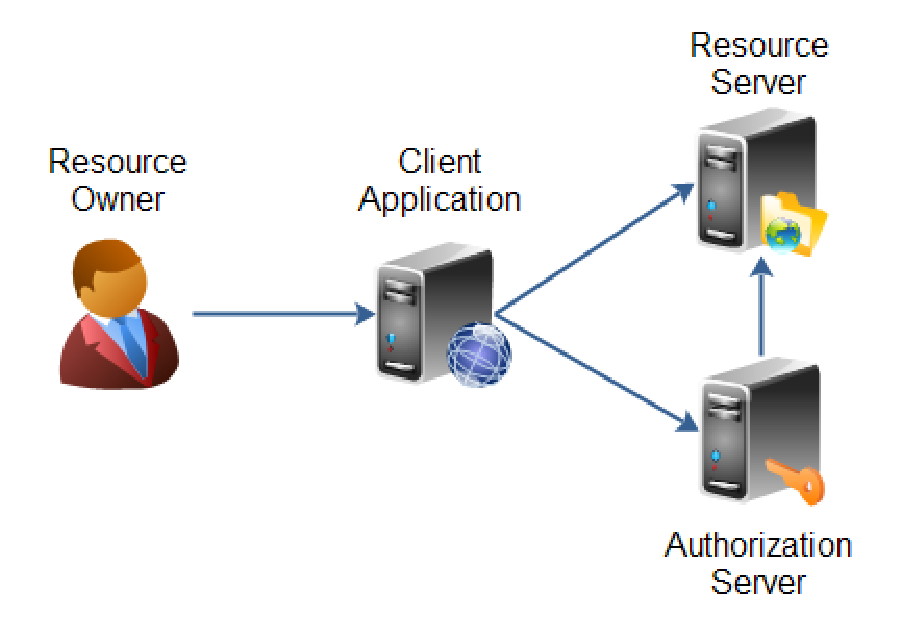
\includegraphics[width=10cm]{overview-roles}
\caption{\-Basic roles defined by \-O\-Auth 2.0}
\end{DoxyImage}
\hypertarget{oauth_flow}{}\section{\-Abstract Protocol Flow}\label{oauth_flow}
\-The basic flow of \-O\-Auth 2.\-0 (as shown in the diagram below) is as follows\-:

\-To get access to protected resources a client sends an authorization request to the resource owner(user). \-If the user grants authorization, the client gets an authorization grant, this grant can take different forms (see \hyperlink{oauth_grant}{\-Authorization \-Grant}) \par
 \-The client exchanges the grant for an access token at the authorization server. \par
 \-The access token can then be used by the client to access the protected resources.

 
\begin{DoxyImage}
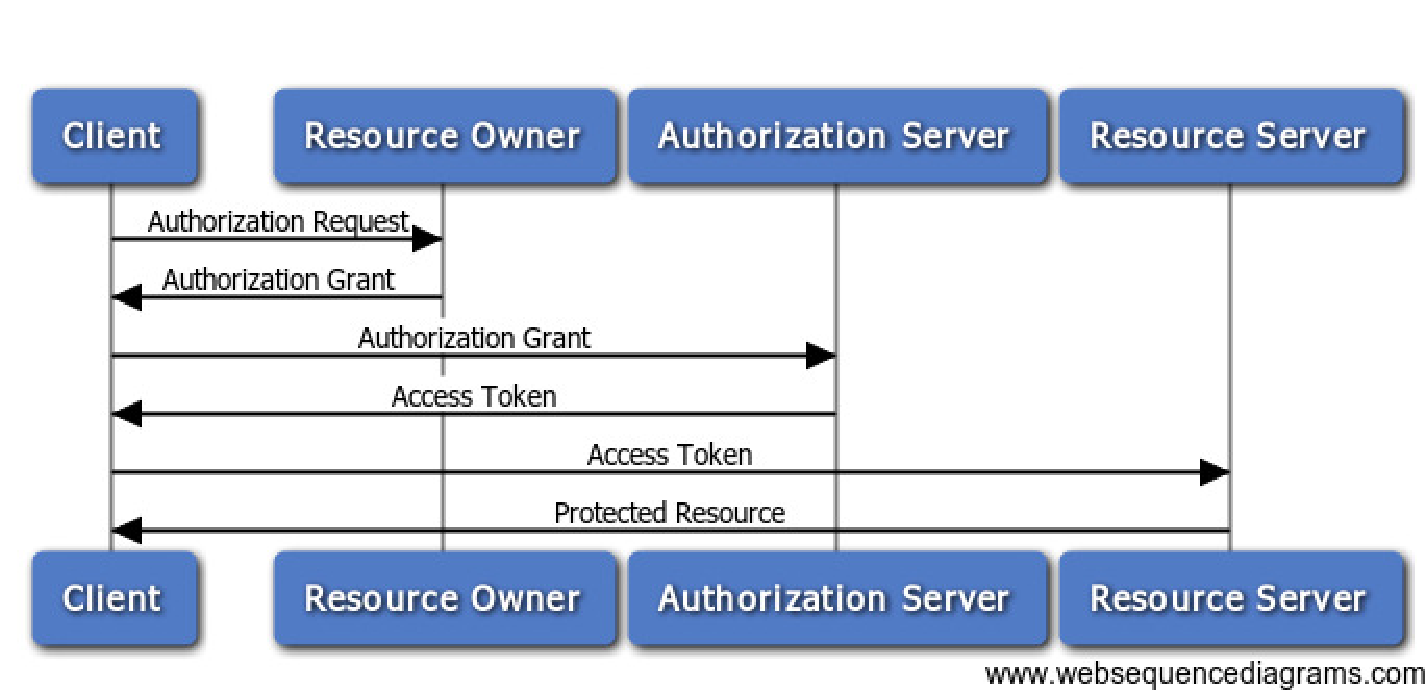
\includegraphics[width=10cm]{flow}
\caption{\-Abstract protocol flow}
\end{DoxyImage}
\hypertarget{oauth_auth}{}\section{\-Authorization}\label{oauth_auth}
\hypertarget{oauth_registration}{}\subsection{\-Registration}\label{oauth_registration}
\-Before the client can request access to protected resources, the client needs to register with the authorization server.\par
 \-During that process the client is assigned a unique client \-I\-D and a client secret.\par
 \-The client also registers a redirect \-U\-R\-I, which is where the user is redirected to, after granting/denying authorization.\par
\hypertarget{oauth_grant}{}\subsection{\-Authorization Grant}\label{oauth_grant}
\-O\-Auth 2.\-0 specifies the following four types of authorization grants\-:\hypertarget{oauth_authcode}{}\subsubsection{\-Authorization Code}\label{oauth_authcode}
\-Since this is the grant implemented in this application a more detailed explanation is required. \par
 \-The basic idea of this grant is as follows\-:
\begin{DoxyItemize}
\item \-The user accesses the client application (1)
\item \-The client app asks the user to log in via an authorization server (2)
\item \-The user is redirected to the authorization server by the client, the client also sends its client \-I\-D along (3)
\item \-After successful login via authorization server the user is asked if he/she wants to grant authorize the client to access the user data.\par
 \-The user is redirected to the registered redirect \-U\-R\-I of the client along with an authorization code (4, 5)
\item \-At the redirect \-U\-R\-I the client connects directly to the authorization server and sends its client \-I\-D, client secret and the authorization code.\par
 \-If all of the data is valid, the authorization server sends back an access token (6, 7)
\item \-This token is sent with every recource request and serves as authentication of the client and authorization to access the recources (10-\/13)
\end{DoxyItemize}

 
\begin{DoxyImage}
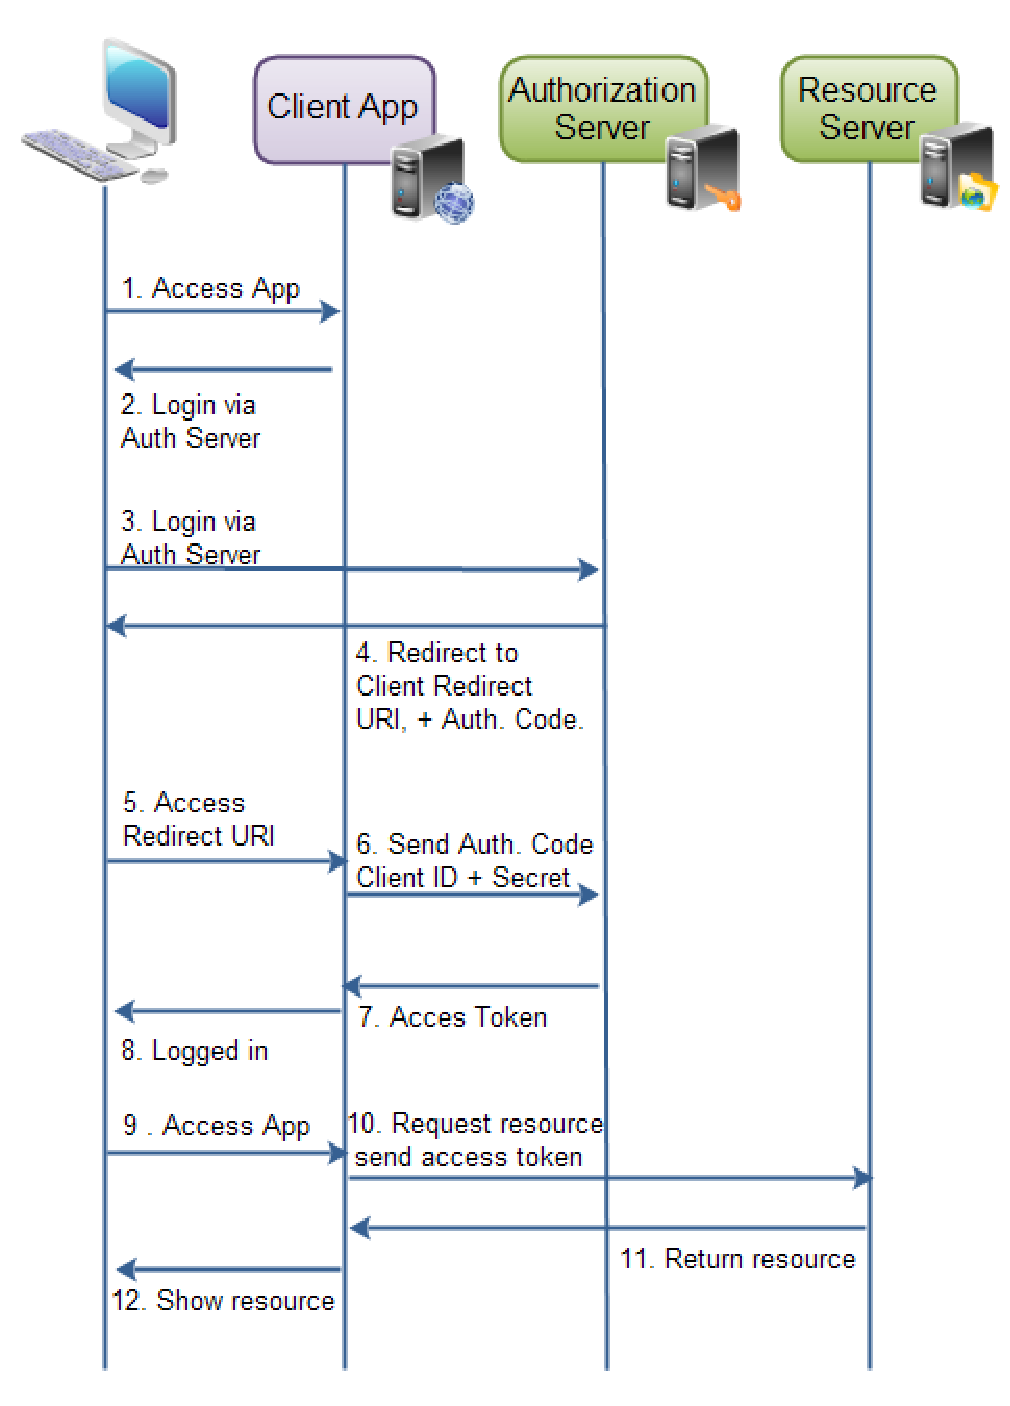
\includegraphics[width=8cm]{authorization-auth-code}
\caption{authorization code grant flow}
\end{DoxyImage}
\hypertarget{oauth_implicit}{}\subsubsection{\-Implicit}\label{oauth_implicit}
\-The implicit grant is similar to authorization code grant, the difference being that the authorization server sends an access token \par
 to the client immediatly after the client logged in and authorized the client.\hypertarget{oauth_ropc}{}\subsubsection{\-Resource Owner Password Credentials}\label{oauth_ropc}
\-This grant requires the user to give the own credentials to the client application, so that the client can use them to access the resources.\hypertarget{oauth_cc}{}\subsubsection{\-Client Credentials}\label{oauth_cc}
\-The authorization server exchanges an access token for client \-I\-D and client secret directly\hypertarget{oauth_endpoint}{}\subsection{\-Endpoint}\label{oauth_endpoint}
\-An endpoint is usually a \-U\-R\-I on a server, in the case of \-O\-Auth 2.\-0 these are\-:
\begin{DoxyItemize}
\item \-The authorization endpoint\-: \par
 \-The endpoint where the user logs in and grants/denies authorization to the client \par
\par

\item \-The redirect endpoint\-: \par
 \-The endpoint where the user is redirected to after granting/denying authorization \par
\par

\item \-The token endpoint\-: \par
 \-The endpoint where the client exchanges client \-I\-D, client secret and authorization code for an access token \par
\par

\end{DoxyItemize}

 
\begin{DoxyImage}
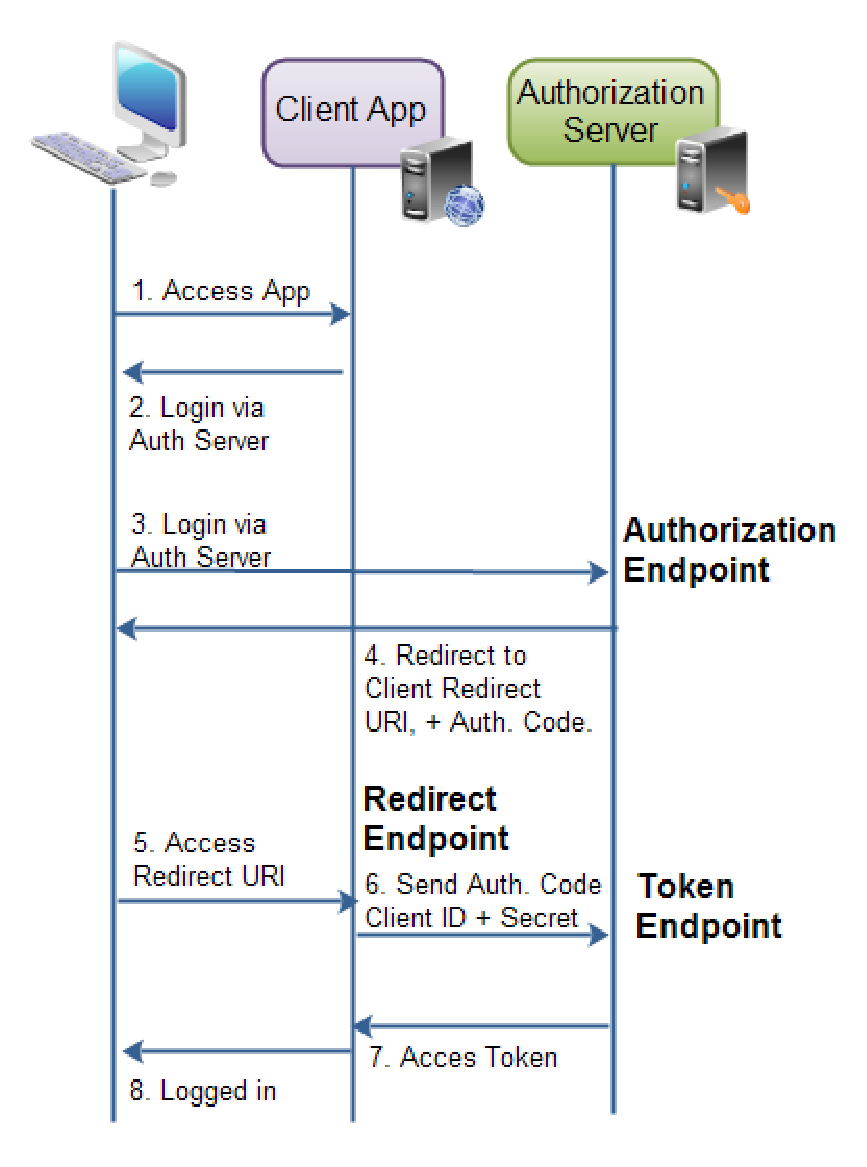
\includegraphics[width=7cm]{endpoints}
\caption{\-Endpoints defined by \-O\-Auth 2.0}
\end{DoxyImage}
 
\chapter{\-Data \-Structure \-Index}
\section{\-Data \-Structures}
\-Here are the data structures with brief descriptions\-:\begin{DoxyCompactList}
\item\contentsline{section}{\hyperlink{class_database}{\-Database} \\*\-Contains functions to simplify database requests }{\pageref{class_database}}{}
\item\contentsline{section}{\hyperlink{class_o_auth_login}{\-O\-Auth\-Login} \\*\-Handles user's login and logout process }{\pageref{class_o_auth_login}}{}
\item\contentsline{section}{\hyperlink{class_registration}{\-Registration} \\*\-Handles the user registration }{\pageref{class_registration}}{}
\end{DoxyCompactList}

\chapter{\-Data \-Structure \-Documentation}
\hypertarget{class_database}{\section{\-Database \-Class \-Reference}
\label{class_database}\index{\-Database@{\-Database}}
}


\-Contains functions to simplify database requests.  


\subsection*{\-Public \-Member \-Functions}
\begin{DoxyCompactItemize}
\item 
\hyperlink{class_database_a095c5d389db211932136b53f25f39685}{\-\_\-\-\_\-construct} ()
\item 
\hyperlink{class_database_a6d8491e0ba1fbe82bbddba3ff5c79468}{get\-User\-Data\-Name} (\$user\-\_\-name)
\item 
\hyperlink{class_database_a6a4a26a4c1f8f44c1f92c240d22c9e03}{get\-User\-Data\-Id} (\$user\-\_\-id)
\item 
\hyperlink{class_database_ad4ce3b281c838afb8f9bb32eaef13188}{get\-Login\-Data} (\$user\-\_\-name)
\item 
\hyperlink{class_database_adfae8c2fdb28633a9ba04e22ea4015c2}{user\-Exists} (\$user\-\_\-name)
\item 
\hyperlink{class_database_a68c8ec601030eabdf057edf4f0cacc58}{add\-User} (\$user\-\_\-name, \$user\-\_\-password\-\_\-hash, \$foaf\-\_\-uri=null)
\item 
\hyperlink{class_database_a729c83344241bddb181c838752a72bbe}{get\-User\-Id} (\$user\-\_\-name)
\item 
\hyperlink{class_database_a9f38c4f4c814e665fc08326a61d4bbb4}{get\-User\-Name} (\$user\-\_\-id)
\item 
\hyperlink{class_database_a35fbecead028c4fa940d0e39a565c137}{get\-User\-Type} (\$user\-\_\-name)
\item 
\hyperlink{class_database_a50dc4c9632a213cd75857e0ea46b79ae}{change\-Entry} (\$user\-\_\-id, \$key, \$value)
\item 
\hyperlink{class_database_ad84e4a2f075fb7fff0aba51ee7db413e}{get\-Scope} (\$user\-\_\-name)
\end{DoxyCompactItemize}
\subsection*{\-Private \-Attributes}
\begin{DoxyCompactItemize}
\item 
\hypertarget{class_database_af908e1ef16f0db5f47519cb83b633e96}{{\bfseries \$db\-\_\-connection} = null}\label{class_database_af908e1ef16f0db5f47519cb83b633e96}

\end{DoxyCompactItemize}


\subsection{\-Detailed \-Description}
\-Contains functions to simplify database requests. 

\begin{DoxyAuthor}{\-Author}
\-Sebastian \-Ankerhold 
\end{DoxyAuthor}


\subsection{\-Constructor \& \-Destructor \-Documentation}
\hypertarget{class_database_a095c5d389db211932136b53f25f39685}{\index{\-Database@{\-Database}!\-\_\-\-\_\-construct@{\-\_\-\-\_\-construct}}
\index{\-\_\-\-\_\-construct@{\-\_\-\-\_\-construct}!Database@{\-Database}}
\subsubsection[{\-\_\-\-\_\-construct}]{\setlength{\rightskip}{0pt plus 5cm}{\bf \-\_\-\-\_\-construct} (
\begin{DoxyParamCaption}
{}
\end{DoxyParamCaption}
)}}\label{class_database_a095c5d389db211932136b53f25f39685}
\-Constructor creates/checks database connection 

\subsection{\-Member \-Function \-Documentation}
\hypertarget{class_database_a68c8ec601030eabdf057edf4f0cacc58}{\index{\-Database@{\-Database}!add\-User@{add\-User}}
\index{add\-User@{add\-User}!Database@{\-Database}}
\subsubsection[{add\-User}]{\setlength{\rightskip}{0pt plus 5cm}{\bf add\-User} (
\begin{DoxyParamCaption}
\item[{\$}]{user\-\_\-name, }
\item[{\$}]{user\-\_\-password\-\_\-hash, }
\item[{\$}]{foaf\-\_\-uri = {\ttfamily null}}
\end{DoxyParamCaption}
)}}\label{class_database_a68c8ec601030eabdf057edf4f0cacc58}
\-Adds a new user and password to the database


\begin{DoxyParams}[1]{\-Parameters}
string & {\em \$user\-\_\-name} & \-The name of a user \\
\hline
string & {\em \$user\-\_\-password\-\_\-hash} & \-The password for that user \\
\hline
\end{DoxyParams}
\begin{DoxyReturn}{\-Returns}
true if adding was successful, else false 
\end{DoxyReturn}
\hypertarget{class_database_a50dc4c9632a213cd75857e0ea46b79ae}{\index{\-Database@{\-Database}!change\-Entry@{change\-Entry}}
\index{change\-Entry@{change\-Entry}!Database@{\-Database}}
\subsubsection[{change\-Entry}]{\setlength{\rightskip}{0pt plus 5cm}{\bf change\-Entry} (
\begin{DoxyParamCaption}
\item[{\$}]{user\-\_\-id, }
\item[{\$}]{key, }
\item[{\$}]{value}
\end{DoxyParamCaption}
)}}\label{class_database_a50dc4c9632a213cd75857e0ea46b79ae}
\-Changes an entry of a given user to a new value


\begin{DoxyParams}[1]{\-Parameters}
int & {\em \$user\-\_\-name} & \-The name of a user \\
\hline
string & {\em \$key} & \-The column that needs changing \\
\hline
string & {\em \$value} & \-The new value of that column \\
\hline
\end{DoxyParams}
\begin{DoxyReturn}{\-Returns}
true if change was successful, false else 
\end{DoxyReturn}
\hypertarget{class_database_ad4ce3b281c838afb8f9bb32eaef13188}{\index{\-Database@{\-Database}!get\-Login\-Data@{get\-Login\-Data}}
\index{get\-Login\-Data@{get\-Login\-Data}!Database@{\-Database}}
\subsubsection[{get\-Login\-Data}]{\setlength{\rightskip}{0pt plus 5cm}{\bf get\-Login\-Data} (
\begin{DoxyParamCaption}
\item[{\$}]{user\-\_\-name}
\end{DoxyParamCaption}
)}}\label{class_database_ad4ce3b281c838afb8f9bb32eaef13188}
\-Returns data necessary for a login


\begin{DoxyParams}[1]{\-Parameters}
string & {\em \$user\-\_\-name} & \-The name of a user \\
\hline
\end{DoxyParams}
\begin{DoxyReturn}{\-Returns}
login relevant data 
\end{DoxyReturn}
\hypertarget{class_database_ad84e4a2f075fb7fff0aba51ee7db413e}{\index{\-Database@{\-Database}!get\-Scope@{get\-Scope}}
\index{get\-Scope@{get\-Scope}!Database@{\-Database}}
\subsubsection[{get\-Scope}]{\setlength{\rightskip}{0pt plus 5cm}{\bf get\-Scope} (
\begin{DoxyParamCaption}
\item[{\$}]{user\-\_\-name}
\end{DoxyParamCaption}
)}}\label{class_database_ad84e4a2f075fb7fff0aba51ee7db413e}
\-Checks the type a given user and returns string of scopes


\begin{DoxyParams}[1]{\-Parameters}
string & {\em \$user\-\_\-name} & \\
\hline
\end{DoxyParams}
\begin{DoxyReturn}{\-Returns}
a string which contains all the scopes the user was permitted 
\end{DoxyReturn}
\hypertarget{class_database_a6a4a26a4c1f8f44c1f92c240d22c9e03}{\index{\-Database@{\-Database}!get\-User\-Data\-Id@{get\-User\-Data\-Id}}
\index{get\-User\-Data\-Id@{get\-User\-Data\-Id}!Database@{\-Database}}
\subsubsection[{get\-User\-Data\-Id}]{\setlength{\rightskip}{0pt plus 5cm}{\bf get\-User\-Data\-Id} (
\begin{DoxyParamCaption}
\item[{\$}]{user\-\_\-id}
\end{DoxyParamCaption}
)}}\label{class_database_a6a4a26a4c1f8f44c1f92c240d22c9e03}
\-Returns all available data of the corresponding user id


\begin{DoxyParams}[1]{\-Parameters}
int & {\em \$user\-\_\-id} & \-The \-I\-D of a user \\
\hline
\end{DoxyParams}
\begin{DoxyReturn}{\-Returns}
all available user data 
\end{DoxyReturn}
\hypertarget{class_database_a6d8491e0ba1fbe82bbddba3ff5c79468}{\index{\-Database@{\-Database}!get\-User\-Data\-Name@{get\-User\-Data\-Name}}
\index{get\-User\-Data\-Name@{get\-User\-Data\-Name}!Database@{\-Database}}
\subsubsection[{get\-User\-Data\-Name}]{\setlength{\rightskip}{0pt plus 5cm}{\bf get\-User\-Data\-Name} (
\begin{DoxyParamCaption}
\item[{\$}]{user\-\_\-name}
\end{DoxyParamCaption}
)}}\label{class_database_a6d8491e0ba1fbe82bbddba3ff5c79468}
\-Returns all available data of the corresponding user name


\begin{DoxyParams}[1]{\-Parameters}
string & {\em \$user\-\_\-name} & \-The name of a user \\
\hline
\end{DoxyParams}
\begin{DoxyReturn}{\-Returns}
all available user data 
\end{DoxyReturn}
\hypertarget{class_database_a729c83344241bddb181c838752a72bbe}{\index{\-Database@{\-Database}!get\-User\-Id@{get\-User\-Id}}
\index{get\-User\-Id@{get\-User\-Id}!Database@{\-Database}}
\subsubsection[{get\-User\-Id}]{\setlength{\rightskip}{0pt plus 5cm}{\bf get\-User\-Id} (
\begin{DoxyParamCaption}
\item[{\$}]{user\-\_\-name}
\end{DoxyParamCaption}
)}}\label{class_database_a729c83344241bddb181c838752a72bbe}
\-Returns the user id of a given user name


\begin{DoxyParams}[1]{\-Parameters}
string & {\em \$user\-\_\-name} & \-The name of a user \\
\hline
\end{DoxyParams}
\begin{DoxyReturn}{\-Returns}
\-The \-I\-D of that user 
\end{DoxyReturn}
\hypertarget{class_database_a9f38c4f4c814e665fc08326a61d4bbb4}{\index{\-Database@{\-Database}!get\-User\-Name@{get\-User\-Name}}
\index{get\-User\-Name@{get\-User\-Name}!Database@{\-Database}}
\subsubsection[{get\-User\-Name}]{\setlength{\rightskip}{0pt plus 5cm}{\bf get\-User\-Name} (
\begin{DoxyParamCaption}
\item[{\$}]{user\-\_\-id}
\end{DoxyParamCaption}
)}}\label{class_database_a9f38c4f4c814e665fc08326a61d4bbb4}
\-Returns the user name of a given user id


\begin{DoxyParams}[1]{\-Parameters}
int & {\em \$user\-\_\-id} & \-The \-Id of a user \\
\hline
\end{DoxyParams}
\begin{DoxyReturn}{\-Returns}
\-The name of that user 
\end{DoxyReturn}
\hypertarget{class_database_a35fbecead028c4fa940d0e39a565c137}{\index{\-Database@{\-Database}!get\-User\-Type@{get\-User\-Type}}
\index{get\-User\-Type@{get\-User\-Type}!Database@{\-Database}}
\subsubsection[{get\-User\-Type}]{\setlength{\rightskip}{0pt plus 5cm}{\bf get\-User\-Type} (
\begin{DoxyParamCaption}
\item[{\$}]{user\-\_\-name}
\end{DoxyParamCaption}
)}}\label{class_database_a35fbecead028c4fa940d0e39a565c137}
\-Returns the user type of a given user name


\begin{DoxyParams}[1]{\-Parameters}
string & {\em \$user\-\_\-name} & \-The name of a user \\
\hline
\end{DoxyParams}
\begin{DoxyReturn}{\-Returns}
\-The type of that user 
\end{DoxyReturn}
\hypertarget{class_database_adfae8c2fdb28633a9ba04e22ea4015c2}{\index{\-Database@{\-Database}!user\-Exists@{user\-Exists}}
\index{user\-Exists@{user\-Exists}!Database@{\-Database}}
\subsubsection[{user\-Exists}]{\setlength{\rightskip}{0pt plus 5cm}{\bf user\-Exists} (
\begin{DoxyParamCaption}
\item[{\$}]{user\-\_\-name}
\end{DoxyParamCaption}
)}}\label{class_database_adfae8c2fdb28633a9ba04e22ea4015c2}
\-Checks if a user with a given name is already registered


\begin{DoxyParams}[1]{\-Parameters}
string & {\em \$user\-\_\-name} & \-The name of a user \\
\hline
\end{DoxyParams}
\begin{DoxyReturn}{\-Returns}
true if user name already exists, otherwise false 
\end{DoxyReturn}


\-The documentation for this class was generated from the following file\-:\begin{DoxyCompactItemize}
\item 
\-Database.\-php\end{DoxyCompactItemize}

\hypertarget{class_o_auth_login}{\section{\-O\-Auth\-Login \-Class \-Reference}
\label{class_o_auth_login}\index{\-O\-Auth\-Login@{\-O\-Auth\-Login}}
}


\-Handles user's login and logout process.  


\subsection*{\-Public \-Member \-Functions}
\begin{DoxyCompactItemize}
\item 
\hyperlink{class_o_auth_login_a8b75ab7c2c6093a8bdc65aae845f94e3}{\-\_\-\-\_\-construct} (\$user\-\_\-name=null)
\item 
\hyperlink{class_o_auth_login_a293fa112652b5448b15c0fb81eafc7cb}{do\-Logout} ()
\item 
\hyperlink{class_o_auth_login_aeb08814a3b11252c66e465a868da3ea7}{is\-User\-Logged\-In} ()
\end{DoxyCompactItemize}
\subsection*{\-Data \-Fields}
\begin{DoxyCompactItemize}
\item 
\hypertarget{class_o_auth_login_ab24faf4aa647cdcee494fc48524ad4ff}{{\bfseries \$errors} = array()}\label{class_o_auth_login_ab24faf4aa647cdcee494fc48524ad4ff}

\item 
\hypertarget{class_o_auth_login_a21a183f927a6d243fe6b4ba3a6c4d4c8}{{\bfseries \$messages} = array()}\label{class_o_auth_login_a21a183f927a6d243fe6b4ba3a6c4d4c8}

\end{DoxyCompactItemize}
\subsection*{\-Private \-Member \-Functions}
\begin{DoxyCompactItemize}
\item 
\hyperlink{class_o_auth_login_a8322cf84e18446c243e58abb037768ff}{check\-Login\-Options} (\$user\-\_\-name=null)
\item 
\hyperlink{class_o_auth_login_aa004457f1cc98762661db58d7c773976}{dologin\-With\-Post\-Data} ()
\item 
\hyperlink{class_o_auth_login_a71b6b746976b1cd18dfc498108e18207}{do\-Login\-With\-Registration\-Data} (\$user\-\_\-name)
\item 
\hyperlink{class_o_auth_login_a51ba603198840f5de5e0c8836a85b5d7}{get\-Auth\-Code} ()
\item 
\hyperlink{class_o_auth_login_a5d251c70a3f9f9daaff7f00ec5f894c0}{get\-Access\-Token} ()
\end{DoxyCompactItemize}
\subsection*{\-Private \-Attributes}
\begin{DoxyCompactItemize}
\item 
\hypertarget{class_o_auth_login_a7691c0162d89de0b6ba47edcd8ba8878}{{\bfseries \$database} = null}\label{class_o_auth_login_a7691c0162d89de0b6ba47edcd8ba8878}

\end{DoxyCompactItemize}


\subsection{\-Detailed \-Description}
\-Handles user's login and logout process. 

\begin{DoxyAuthor}{\-Author}
\-Sebastian \-Ankerhold 
\end{DoxyAuthor}


\subsection{\-Constructor \& \-Destructor \-Documentation}
\hypertarget{class_o_auth_login_a8b75ab7c2c6093a8bdc65aae845f94e3}{\index{\-O\-Auth\-Login@{\-O\-Auth\-Login}!\-\_\-\-\_\-construct@{\-\_\-\-\_\-construct}}
\index{\-\_\-\-\_\-construct@{\-\_\-\-\_\-construct}!OAuthLogin@{\-O\-Auth\-Login}}
\subsubsection[{\-\_\-\-\_\-construct}]{\setlength{\rightskip}{0pt plus 5cm}{\bf \-\_\-\-\_\-construct} (
\begin{DoxyParamCaption}
\item[{\$}]{user\-\_\-name = {\ttfamily null}}
\end{DoxyParamCaption}
)}}\label{class_o_auth_login_a8b75ab7c2c6093a8bdc65aae845f94e3}
\-Constructor \-Checks and performs the possible login actions 

\subsection{\-Member \-Function \-Documentation}
\hypertarget{class_o_auth_login_a8322cf84e18446c243e58abb037768ff}{\index{\-O\-Auth\-Login@{\-O\-Auth\-Login}!check\-Login\-Options@{check\-Login\-Options}}
\index{check\-Login\-Options@{check\-Login\-Options}!OAuthLogin@{\-O\-Auth\-Login}}
\subsubsection[{check\-Login\-Options}]{\setlength{\rightskip}{0pt plus 5cm}{\bf check\-Login\-Options} (
\begin{DoxyParamCaption}
\item[{\$}]{user\-\_\-name = {\ttfamily null}}
\end{DoxyParamCaption}
)\hspace{0.3cm}{\ttfamily  \mbox{[}private\mbox{]}}}}\label{class_o_auth_login_a8322cf84e18446c243e58abb037768ff}
\-Checks the \-G\-E\-T and \-P\-O\-S\-T data and performs the corresponding actions.


\begin{DoxyParams}[1]{\-Parameters}
string & {\em \$user\-\_\-name} & \-The name of a user \\
\hline
\end{DoxyParams}
\hypertarget{class_o_auth_login_aa004457f1cc98762661db58d7c773976}{\index{\-O\-Auth\-Login@{\-O\-Auth\-Login}!dologin\-With\-Post\-Data@{dologin\-With\-Post\-Data}}
\index{dologin\-With\-Post\-Data@{dologin\-With\-Post\-Data}!OAuthLogin@{\-O\-Auth\-Login}}
\subsubsection[{dologin\-With\-Post\-Data}]{\setlength{\rightskip}{0pt plus 5cm}{\bf dologin\-With\-Post\-Data} (
\begin{DoxyParamCaption}
{}
\end{DoxyParamCaption}
)\hspace{0.3cm}{\ttfamily  \mbox{[}private\mbox{]}}}}\label{class_o_auth_login_aa004457f1cc98762661db58d7c773976}
\-Log in with post data by checking the validity of posted data and store essential data into \-P\-H\-P \-S\-E\-S\-S\-I\-O\-N \hypertarget{class_o_auth_login_a71b6b746976b1cd18dfc498108e18207}{\index{\-O\-Auth\-Login@{\-O\-Auth\-Login}!do\-Login\-With\-Registration\-Data@{do\-Login\-With\-Registration\-Data}}
\index{do\-Login\-With\-Registration\-Data@{do\-Login\-With\-Registration\-Data}!OAuthLogin@{\-O\-Auth\-Login}}
\subsubsection[{do\-Login\-With\-Registration\-Data}]{\setlength{\rightskip}{0pt plus 5cm}{\bf do\-Login\-With\-Registration\-Data} (
\begin{DoxyParamCaption}
\item[{\$}]{user\-\_\-name}
\end{DoxyParamCaption}
)\hspace{0.3cm}{\ttfamily  \mbox{[}private\mbox{]}}}}\label{class_o_auth_login_a71b6b746976b1cd18dfc498108e18207}
\-If a user registered a new account, this function uses the entered data to log in the user


\begin{DoxyParams}{\-Parameters}
{\em } & \\
\hline
\end{DoxyParams}
\hypertarget{class_o_auth_login_a293fa112652b5448b15c0fb81eafc7cb}{\index{\-O\-Auth\-Login@{\-O\-Auth\-Login}!do\-Logout@{do\-Logout}}
\index{do\-Logout@{do\-Logout}!OAuthLogin@{\-O\-Auth\-Login}}
\subsubsection[{do\-Logout}]{\setlength{\rightskip}{0pt plus 5cm}{\bf do\-Logout} (
\begin{DoxyParamCaption}
{}
\end{DoxyParamCaption}
)}}\label{class_o_auth_login_a293fa112652b5448b15c0fb81eafc7cb}
\-Performs the logout by resetting the \$\-\_\-\-S\-E\-S\-S\-I\-O\-N array and displays a logout message \hypertarget{class_o_auth_login_a5d251c70a3f9f9daaff7f00ec5f894c0}{\index{\-O\-Auth\-Login@{\-O\-Auth\-Login}!get\-Access\-Token@{get\-Access\-Token}}
\index{get\-Access\-Token@{get\-Access\-Token}!OAuthLogin@{\-O\-Auth\-Login}}
\subsubsection[{get\-Access\-Token}]{\setlength{\rightskip}{0pt plus 5cm}{\bf get\-Access\-Token} (
\begin{DoxyParamCaption}
{}
\end{DoxyParamCaption}
)\hspace{0.3cm}{\ttfamily  \mbox{[}private\mbox{]}}}}\label{class_o_auth_login_a5d251c70a3f9f9daaff7f00ec5f894c0}
\-Request an access token by sending the received auth.\-code to the token endpoint. \-If successful the token will be stored in \-S\-E\-S\-S\-I\-O\-N \hypertarget{class_o_auth_login_a51ba603198840f5de5e0c8836a85b5d7}{\index{\-O\-Auth\-Login@{\-O\-Auth\-Login}!get\-Auth\-Code@{get\-Auth\-Code}}
\index{get\-Auth\-Code@{get\-Auth\-Code}!OAuthLogin@{\-O\-Auth\-Login}}
\subsubsection[{get\-Auth\-Code}]{\setlength{\rightskip}{0pt plus 5cm}{\bf get\-Auth\-Code} (
\begin{DoxyParamCaption}
{}
\end{DoxyParamCaption}
)\hspace{0.3cm}{\ttfamily  \mbox{[}private\mbox{]}}}}\label{class_o_auth_login_a51ba603198840f5de5e0c8836a85b5d7}
\-Redirects to the authorization endpoint to request an authorization code \-If successful the user will be redirected back to this location with a code \hypertarget{class_o_auth_login_aeb08814a3b11252c66e465a868da3ea7}{\index{\-O\-Auth\-Login@{\-O\-Auth\-Login}!is\-User\-Logged\-In@{is\-User\-Logged\-In}}
\index{is\-User\-Logged\-In@{is\-User\-Logged\-In}!OAuthLogin@{\-O\-Auth\-Login}}
\subsubsection[{is\-User\-Logged\-In}]{\setlength{\rightskip}{0pt plus 5cm}{\bf is\-User\-Logged\-In} (
\begin{DoxyParamCaption}
{}
\end{DoxyParamCaption}
)}}\label{class_o_auth_login_aeb08814a3b11252c66e465a868da3ea7}
\-Simply return the current state of the user's login \begin{DoxyReturn}{\-Returns}
boolean user's login status 
\end{DoxyReturn}


\-The documentation for this class was generated from the following file\-:\begin{DoxyCompactItemize}
\item 
\-O\-Auth\-Login.\-php\end{DoxyCompactItemize}

\hypertarget{class_registration}{\section{\-Registration \-Class \-Reference}
\label{class_registration}\index{\-Registration@{\-Registration}}
}


\-Handles the user registration.  


\subsection*{\-Public \-Member \-Functions}
\begin{DoxyCompactItemize}
\item 
\hyperlink{class_registration_a095c5d389db211932136b53f25f39685}{\-\_\-\-\_\-construct} ()
\end{DoxyCompactItemize}
\subsection*{\-Data \-Fields}
\begin{DoxyCompactItemize}
\item 
\hypertarget{class_registration_ab24faf4aa647cdcee494fc48524ad4ff}{{\bfseries \$errors} = array()}\label{class_registration_ab24faf4aa647cdcee494fc48524ad4ff}

\item 
\hypertarget{class_registration_a21a183f927a6d243fe6b4ba3a6c4d4c8}{{\bfseries \$messages} = array()}\label{class_registration_a21a183f927a6d243fe6b4ba3a6c4d4c8}

\end{DoxyCompactItemize}
\subsection*{\-Private \-Member \-Functions}
\begin{DoxyCompactItemize}
\item 
\hyperlink{class_registration_a5e4143fb94f6541b6b88503a9905d4e5}{register\-New\-User} ()
\end{DoxyCompactItemize}
\subsection*{\-Private \-Attributes}
\begin{DoxyCompactItemize}
\item 
\hypertarget{class_registration_a7691c0162d89de0b6ba47edcd8ba8878}{{\bfseries \$database} = null}\label{class_registration_a7691c0162d89de0b6ba47edcd8ba8878}

\end{DoxyCompactItemize}


\subsection{\-Detailed \-Description}
\-Handles the user registration. 

\begin{DoxyAuthor}{\-Author}
\-Sebastian \-Ankerhold 
\end{DoxyAuthor}


\subsection{\-Constructor \& \-Destructor \-Documentation}
\hypertarget{class_registration_a095c5d389db211932136b53f25f39685}{\index{\-Registration@{\-Registration}!\-\_\-\-\_\-construct@{\-\_\-\-\_\-construct}}
\index{\-\_\-\-\_\-construct@{\-\_\-\-\_\-construct}!Registration@{\-Registration}}
\subsubsection[{\-\_\-\-\_\-construct}]{\setlength{\rightskip}{0pt plus 5cm}{\bf \-\_\-\-\_\-construct} (
\begin{DoxyParamCaption}
{}
\end{DoxyParamCaption}
)}}\label{class_registration_a095c5d389db211932136b53f25f39685}
\-Constructor 

\subsection{\-Member \-Function \-Documentation}
\hypertarget{class_registration_a5e4143fb94f6541b6b88503a9905d4e5}{\index{\-Registration@{\-Registration}!register\-New\-User@{register\-New\-User}}
\index{register\-New\-User@{register\-New\-User}!Registration@{\-Registration}}
\subsubsection[{register\-New\-User}]{\setlength{\rightskip}{0pt plus 5cm}{\bf register\-New\-User} (
\begin{DoxyParamCaption}
{}
\end{DoxyParamCaption}
)\hspace{0.3cm}{\ttfamily  \mbox{[}private\mbox{]}}}}\label{class_registration_a5e4143fb94f6541b6b88503a9905d4e5}
\-Handles the entire registration process. \-Checks all error possibilities ,creates a new user in the database and performs a login for the new user if everything is fine. 

\-The documentation for this class was generated from the following file\-:\begin{DoxyCompactItemize}
\item 
\-Registration.\-php\end{DoxyCompactItemize}

\printindex
\end{document}
